% thesis-template-english.tex - English Academic Thesis Template for German Universities
% This template follows German academic conventions with English content:
% - German university title page format
% - Front matter organization (TOC, abstracts, lists, glossary)
% - Required German abstract (Zusammenfassung) + English abstract
% - Standard book class for maximum flexibility
% - IEEE bibliography style for international compatibility
% 
% IMPORTANT: Always verify compliance with your specific institution's guidelines
% 
% Template structure: German academic convention with thoughtful front/back matter organization
\documentclass[oneside,11pt]{book}


% Encoding and languages - English primary, German secondary for abstracts
\usepackage[utf8]{inputenc}
\usepackage[T1]{fontenc}
\usepackage[english]{babel} % English as main language
\usepackage[autostyle]{csquotes}


% Basic Math
\usepackage{amsmath, amssymb, amsthm}

% Graphics
\usepackage{graphicx}

% Bibliography - International style
\usepackage[backend=biber, style=ieee]{biblatex} % IEEE style for international appeal
\addbibresource{thesis_references.bib}

% Load hyperref BEFORE glossaries
\usepackage[hidelinks,hyperfootnotes=false]{hyperref}
\hypersetup{
    pdftitle={Your Thesis Title},
    pdfauthor={Marlin Jai Pohl},
    pdfsubject={Bachelor Thesis},
    pdfkeywords={thesis, bachelor, computer science}
}

% Glossary and abbreviations - now included in TOC automatically
\usepackage[toc,acronym,nonumberlist,nogroupskip]{glossaries}
\makeglossaries

% Set glossary style to simple list format (single column, rows)
\setglossarystyle{list}

% Include glossary entries
% glossary-entries.tex - Contains all glossary entries for the thesis
% This file is included in the main document to define all glossary terms

% Regular glossary entries
\newglossaryentry{staticweb}{
    name=Static Code Output,
    description={Traditional web content consisting of HTML, CSS, and JavaScript files that are pre-built and served as-is, without dynamic server-side processing and without the need for a server-side language like PHP or Node.js}
}

\newglossaryentry{Framework}{
    name=Framework,
    description={A software framework that provides a foundation for developing applications by offering reusable code and standardized programming interfaces}
}

\newglossaryentry{algorithm}{
    name=Algorithm,
    description={A step-by-step procedure or formula for solving a problem or completing a task}
}

% Abbreviation entries - using regular glossary entries to show both forms
\newglossaryentry{API}{
    name=API (Application Programming Interface),
    description={A set of protocols and tools for building software applications that specifies how software components should interact}
}

\newglossaryentry{ML}{
    name=ML (Machine Learning),
    description={A subset of artificial intelligence that enables computers to learn and improve from experience without being explicitly programmed}
}

\newglossaryentry{SPA}{
    name=SPA (Single Page Application),
    description={A web application that allows users to navigate through a single page without reloading the page, providing a more fluid user experience}
}

\newglossaryentry{WYSIWYG}{
    name=WYSIWYG (What You See Is What You Get),
    description={A technology that allows users to create and edit content visually, without the need for coding, where the editing interface closely resembles the final output}
}

\newglossaryentry{CMS}{
    name=CMS (Content Management System),
    description={A software system that allows users to create, manage, and publish content without the need for technical knowledge}
}

\newglossaryentry{GDPR}{
    name=GDPR (General Data Protection Regulation),
    description={A regulation that protects the personal data of individuals within the European Union}
} 

\newglossaryentry{UI}{
    name=UI (User Interface),
    description={The graphical interface that allows users to interact with a computer system}
}

\newglossaryentry{meta-programming}{
    name=Meta-programming,
    description={A programming paradigm that allows a program to generate other programs, in specific SPAs during \gls{runtime}}
}

\newglossaryentry{compile-time}{
    name=Compile-time,
    description={The time during which a program is compiled, including the time it takes to compile the program}
}

\newglossaryentry{runtime}{
    name=Runtime,
    description={The time during which a program is running, including the time it takes to execute the program}
}

% Code Listings
\usepackage{listings}
\lstset{
  basicstyle=\footnotesize\ttfamily,
  frame=single,
  breaklines=true,
  numbers=left,
  numberstyle=\tiny,
  captionpos=b,
  language=Python % Default language, change as needed
}

% Tables and Captions
\usepackage{booktabs}
\usepackage[small, labelfont=bf]{caption}


% Page layout
\usepackage[hmargin=3cm, top=2.5cm, bottom=2.5cm]{geometry}

% TOC and heading customization
\usepackage{titlesec}

\usepackage{tocloft}
\renewcommand{\cftbeforechapskip}{.8em}
\renewcommand{\cftbeforesecskip}{0.3em}
\renewcommand{\cftbeforesubsecskip}{0.3em}
\renewcommand{\cftbeforesubsubsecskip}{0.3em}


% Format all heading levels consistently - KOMA-Script style
\titleformat{\chapter}
  {\normalfont\LARGE\bfseries}
  {\thechapter.}
  {0.5em}
  {}

\titleformat{\section}
  {\normalfont\Large\bfseries}
  {\thesection}
  {0.5em}
  {}

\titleformat{\subsection}
  {\normalfont\large\bfseries}
  {\thesubsection}
  {0.5em}
  {}

\titleformat{\subsubsection}
  {\normalfont\normalsize\bfseries}
  {\thesubsubsection}
  {0.5em}
  {}

% Add spacing between sections - KOMA-Script style
\titlespacing*{\chapter}{0pt}{0pt}{1em}
\titlespacing*{\section}{0pt}{1em}{1em}
\titlespacing*{\subsection}{0pt}{1em}{1em}
\titlespacing*{\subsubsection}{0pt}{1em}{1em}


% Save the original \tableofcontents after all packages are loaded
\let\oldtableofcontents\tableofcontents

% Redefine \tableofcontents to use smaller font and restore heading logic
\renewcommand{\tableofcontents}{%
  {\small
    \oldtableofcontents
  }%
  \renewcommand{\contentsname}{}%
}

% KOMA-Script style page numbering
\usepackage{fancyhdr}
\pagestyle{fancy}
\fancyhf{}
\renewcommand{\headrulewidth}{0pt}
\renewcommand{\footrulewidth}{0pt}
\fancyfoot[C]{\thepage}

% Front matter page style
\fancypagestyle{frontmatter}{
  \fancyhf{}
  \renewcommand{\headrulewidth}{0pt}
  \renewcommand{\footrulewidth}{0pt}
  \fancyfoot[C]{\roman{page}}
}

% Main matter page style
\fancypagestyle{mainmatter}{
  \fancyhf{}
  \renewcommand{\headrulewidth}{0pt}
  \renewcommand{\footrulewidth}{0pt}
  \fancyfoot[C]{\arabic{page}}
}

% Apply front matter style to front matter
\let\oldfrontmatter\frontmatter
\renewcommand{\frontmatter}{
  \oldfrontmatter
  \pagestyle{frontmatter}
}

% Apply main matter style to main matter
\let\oldmainmatter\mainmatter
\renewcommand{\mainmatter}{
  \oldmainmatter
  \pagestyle{mainmatter}
}

% Ensure consistent spacing and depth
\setcounter{tocdepth}{3}
\setcounter{secnumdepth}{3}

% Consistent link colors
\hypersetup{
    colorlinks=true,
    linkcolor=black,
    filecolor=black,
    urlcolor=black,
    citecolor=black,
    pdftitle={Your Thesis Title},
    pdfauthor={Marlin Jai Pohl},
    pdfsubject={Bachelor Thesis},
    pdfkeywords={thesis, bachelor, computer science}
}

\setlength{\parskip}{1em}
\setlength{\parindent}{0pt}

% Theorems, Definitions, etc. - English names

% Theorem - Used to state and prove important mathematical/scientific claims that need formal proof
\newtheorem{theorem}{Theorem}[chapter]

% Definition - Used to formally define new terms, concepts or notations
\newtheorem{definition}[theorem]{Definition}

% Lemma - Used for supporting theorems/propositions that are needed to prove a larger theorem
\newtheorem{lemma}[theorem]{Lemma}

% Remark - Used to make observations, notes or comments about previous statements
\newtheorem{remark}[theorem]{Remark}

% Corollary - Used for results that follow directly from a previously proven theorem
\newtheorem{corollary}[theorem]{Corollary}

% Example - Used to provide concrete instances or illustrations of concepts
\newtheorem{example}[theorem]{Example}

% Document metadata
\title{A Multi-Layered Visual Application Builder with Dynamic CSS Class Generation based on a VDOM centric meta-programming approach}
\author{Marlin Jai Pohl}
\date{\today}

\hyphenpenalty=5000
\exhyphenpenalty=5000

%\usepackage{mathptmx} % Times font
\usepackage{helvet} \renewcommand{\familydefault}{\sfdefault}

% Document
\begin{document}

% Title page - German university format with English content
\begin{titlepage}
\centering
\vfill

\includegraphics[width=0.5\textwidth]{HTW_Berlin_Logo_farbig.jpg}
\vspace{1cm}

{\Large
  \setlength{\baselineskip}{1.5em} % or try 2em for more space
  \textbf{
    A Multi-Layered Visual Application Builder \\
    with Dynamic CSS Class Generation \\
  }
}
\vfill

Bachelor Thesis\\
\vspace{0.5cm}
submitted in partial fulfillment of the requirements\\
for the degree of\\
\vspace{0.5cm}
\textbf{Bachelor of Science (B.Sc.)}\\
\vspace{0.5cm}
at\\
\vspace{0.5cm}
Berlin University of Applied Sciences\\
Faculty 4: Computer Science, Communication and Economics\\
Study Program \textit{International Media and Computing}

\vspace{2cm}

% Centered supervisor information
\begin{center}
  \begin{tabular}{@{}l@{\hspace{0.5cm}}l@{}}
    First Supervisor: & Academic Title First Name Last Name \\
    Second Supervisor: & Academic Title First Name Last Name
  \end{tabular}
\end{center}

\vspace{2cm}

Submitted by: Your Full Name [Student ID]\\
Berlin, \today

\vfill
\end{titlepage}

% Front matter - German academic structure
\frontmatter

% Table of contents and lists - German convention (front matter)

\chapter*{Abstract}
\addcontentsline{toc}{chapter}{Abstract}

% English abstract
When faced with the challenge of creating content and interactive web experiences, less technical users have to rely on \gls{CMS} like WordPress and \gls{WYSIWYG} editors.


Although these tools partially satisfy the needs of modern web experiences, many of them have limitations regarding the \gls{staticweb} they produce, and an inaccuracy between the preview layer and the final rendered content in the Web browser.


Due to the static output of tools like Webflow, WordPress, Wix, etc., users cannot make use of the \gls{SPA} features that come with modern JavaScript frameworks like React, NextJS or VueJS, which are based on the dynamic injection of JavaScript code during \gls{runtime}.


The following thesis answers the question of how a multilayered visual application builder allowing real-time \gls{UI} editing, dynamic CSS class generation, and multi-touch interactions can be implemented using the modern JavaScript framework NextJS. 

As a result, the barrier of entry to build great software is lowered by applying the concepts of meta-programming.

The concept of meta programming is defined as follows:

% TODO: ask if this is correct
"Meta-programs analyze, generate, and transform object programs. In this process, object programs are structured data."\footfullcite[p. 299]{visser2002}

In the context of this thesis, meta-programming is used to implement a program that dynamically generates other programs, in specific SPAs during \gls{runtime}, by using a component based approach with drag and drop functionality and real-time \gls{UI} editing.

% Main content
\mainmatter

\chapter{Introduction}
\label{ch:introduction}

% 1.1 Visual Application Builder Overview
\section{Visual Application Builder Overview}
\label{sec:visual-builder-overview}

This thesis presents a \textbf{multi-layered visual application builder} that enables real-time \gls{UI} editing while maintaining full React functionality. The system consists of four integrated interface layers working in concert to provide comprehensive visual development capabilities:

\begin{enumerate}
    \item \textbf{Component Palette}: Drag-and-drop library of available UI components
    \item \textbf{Canvas with Responsive Preview}: Main editing area with desktop, tablet, and mobile viewports
    \item \textbf{Layers Panel}: Hierarchical tree view of component structure and relationships
    \item \textbf{Properties Panel}: Dynamic style and behavior editor for selected components
\end{enumerate}

\begin{figure}[h]
    \centering
    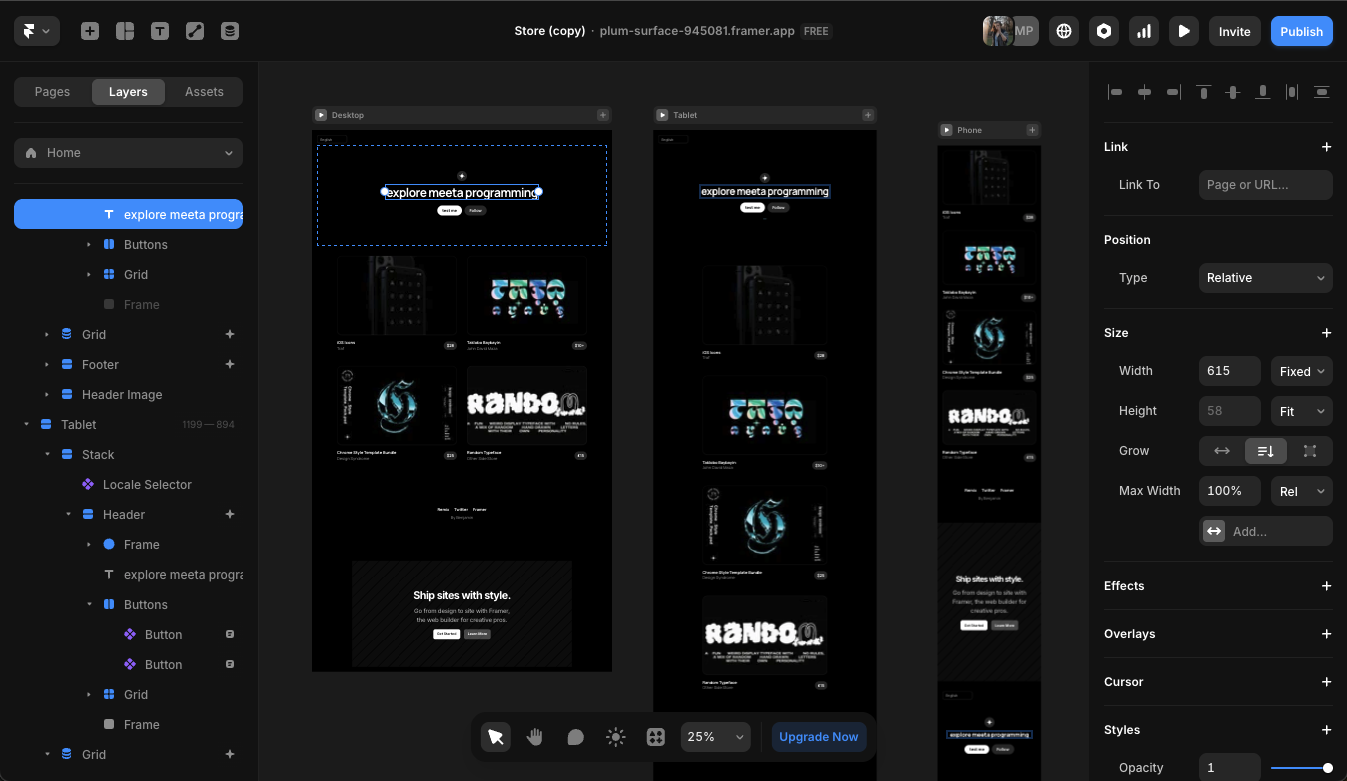
\includegraphics[width=0.95\textwidth]{images/Framer_multi_device_interface.png}
    \caption{Framer Interface showing multi-layered visual editing environment with layers panel (left), responsive canvas (center), properties panel (right), and component palette (top - currently not shown)\cite{framer}}
    \label{fig:framer-interface}
\end{figure}

As demonstrated in Figure~\ref{fig:framer-interface}, existing tools like Framer already implement variations of this multi-layered approach, showing the practical viability of such interfaces for visual application development.


% 1.2 Multi-Layered Interface Architecture
\newpage
\section{Multi-Layered Interface Architecture}
\label{sec:interface-architecture}

\subsection{Component Palette and Canvas Integration}

The \textbf{component palette} provides a library of reusable UI elements—buttons, forms, containers, text components—that users drag onto the main \textbf{canvas}. Unlike traditional drag-and-drop builders that generate static markup, this system creates dynamic component configurations that maintain React's interactive capabilities.

The \textbf{canvas} serves as the primary visual editing surface, featuring three responsive preview modes:

\begin{itemize}
    \item \textbf{Desktop View}: Full-width layout for standard web applications
    \item \textbf{Tablet View}: Medium-width responsive breakpoint (768px-1024px)
    \item \textbf{Mobile View}: Narrow layout for mobile-optimized interfaces (<768px)
\end{itemize}

Each viewport provides real-time preview of how the application will appear across different device types, with responsive styling automatically managed through the visual interface.

\subsection{Layers Panel: Component Tree Management}

The \textbf{layers panel} presents a hierarchical tree view of the component structure, enabling users to:

\begin{itemize}
    \item Navigate complex nested component relationships
    \item Reorder components through drag-and-drop operations
    \item Select components for editing without clicking on the canvas
    \item Manage component visibility and locking states
    \item Organize components into logical groupings
\end{itemize}

This panel reflects the underlying \textbf{component tree model}—a serializable data structure that maintains the complete application state including component relationships, properties, and interaction definitions.

\newpage
\subsection{Properties Panel: Dynamic Component Configuration}

The \textbf{properties panel} provides context-sensitive editing interfaces that adapt based on the currently selected component type. For each component, users can configure:

\begin{itemize}
    \item \textbf{Visual Styles}: Colors, typography, spacing, layout properties through intuitive controls
    \item \textbf{Content}: Text, images, and media through direct editing interfaces
    \item \textbf{Component State}: Initial values for interactive elements (form inputs, counters, toggles)
    \item \textbf{Interactions}: Click handlers, hover effects, and user-defined JavaScript actions
    \item \textbf{Responsive Behavior}: Device-specific styling and layout adaptations
\end{itemize}

The panel dynamically generates appropriate input controls—color pickers for colors, number inputs for dimensions, dropdown menus for predefined options—based on the selected component's schema.

% 1.3 The Challenge: Bridging Visual Editing and Runtime Interactivity
\section{The Challenge: Bridging Visual Editing and\\Runtime Interactivity}
\label{sec:bridging-challenge}

The fundamental challenge addressed by this thesis lies in maintaining \textbf{two distinct reactive systems} that must work in perfect synchronization:

\subsection{System 1: Editor Reactivity}
The visual editor interface requires real-time updates when users:
\begin{itemize}
    \item Drag components between layers
    \item Modify styles in the properties panel
    \item Select different components for editing
    \item Switch between responsive breakpoints
\end{itemize}

These operations must immediately reflect in all interface layers—the canvas preview, layers panel, and properties panel—ensuring consistent visual feedback during the editing process.

\subsection{System 2: Runtime Component Interactivity}
Simultaneously, the components being edited must maintain their intended runtime behavior:
\begin{itemize}
    \item Buttons must handle click events and update their state
    \item Forms must manage input validation and submission
    \item Interactive elements must respond to user interactions
    \item Component state must persist and update appropriately
\end{itemize}

This runtime interactivity must function both in the live preview during editing and in the final exported application.

% 1.4 Research Questions and Technical Objectives
\section{Research Questions and Technical Objectives}
\label{sec:research-objectives}

\textbf{Primary Research Question:}

How can a multi-layered visual interface enable real-time application building while maintaining full React interactivity through a meta-programming approach that transforms editor configurations into functional \gls{SPA} components?

\textbf{Supporting Research Questions:}

\begin{itemize}
    \item How can the four interface layers (palette, canvas, layers, properties) synchronize in real-time during visual editing operations?
    \item What architectural patterns enable seamless transformation from static component configurations to interactive React components?
    \item How can visual interfaces make complex component state management and interactions accessible to non-technical users?
\end{itemize}

\textbf{Technical Objectives:}

\begin{enumerate}
    \item Design and implement a unified component tree model that supports both visual editing and React export capabilities
    \item Develop responsive preview systems that maintain consistent behavior across desktop, tablet, and mobile viewports
    \item Create dynamic property editing interfaces that adapt to different component types and interaction patterns
    \item Implement real-time synchronization between all interface layers during editing operations
\end{enumerate}

% 1.5 Contribution and Innovation
\section{Contribution and Innovation}
\label{sec:contribution}

This thesis makes several key contributions to the field of visual web application development:

\begin{enumerate}
    \item \textbf{Multi-Layered Interface Architecture}: A comprehensive visual editing environment that maintains professional development workflow patterns while remaining accessible to non-technical users
    
    \item \textbf{Dual Reactive Systems Integration}: Novel architecture separating editor reactivity (MobX-State-Tree) from runtime component reactivity (React state) while maintaining seamless synchronization
    
    \item \textbf{Meta-Programming Component Generation}: Generic transformation patterns that convert visual editor configurations into fully functional React applications with maintained interactivity
    
    \item \textbf{Responsive-First Visual Design}: Integrated multi-viewport editing that enables device-specific optimization during the visual design process
\end{enumerate}

The resulting system demonstrates how visual application builders can provide professional-grade development capabilities while maintaining the accessibility and immediate feedback that make visual editing powerful for rapid prototyping and non-technical content creation.

% 1.6 Thesis Structure
\section{Thesis Structure}
\label{sec:structure}

This thesis is organized into the following chapters:

\textbf{Chapter 2: Foundations} establishes the theoretical and technological groundwork, including an analysis of existing visual building tools, React architecture patterns, meta-programming concepts, and related academic research.

\textbf{Chapter 3: System Design and Architecture} describes the multi-layered architecture, component models, state management patterns, and technical design decisions.

\textbf{Chapter 4: Implementation} provides detailed coverage of the implementation process, including core algorithms, user interface design, and integration challenges.

\textbf{Chapter 5: Evaluation and Testing} presents performance analysis, usability testing results, and comparative evaluation against existing solutions.

\textbf{Chapter 6: Conclusion and Future Work} summarizes the research findings, discusses limitations, and outlines opportunities for future development.

% Print unified glossary before references
\printglossaries


\end{document}
